\documentclass[uct_visualisation_thesis.tex]{subfiles}

Prezentowany system, poza tytułowym algorytmem UCT, wykorzystuje również usprawniony algorytm Walkera do wizualizacji drzew. W rozdziałach \ref{subsec:uct} i \ref{subsec:tree_vis} zostały przedstawione zagadnienia teoretyczne z zakresu obu algorytmów.

\section{Algorytmy MCTS} \label{subsec:mcts_group}
Monte-Carlo Tree Search to heurystyka, której celem jest podejmowanie decyzji w pewnych zadaniach sztucznej inteligencji, na przykład wybieranie ruchów w grach. Metoda jest oparta na przeszukiwaniu możliwych stanów gry zapisanych w wierzchołkach drzewa i losowym symulowaniu rozgrywek. Algorytmy MCTS opierają się na rozbudowywaniu drzewa ze stanami gry przez iteracyjne wykonywanie czterech faz. Jednym z najpowszechniejszych wariantów MCTS jest algorytm UCT. Pseudokod opisany w Listingu \ref{lst:mcts} oraz implementacja MCTS w projekcie bazują na \cite{banditbased}. Przykład działania algorytmu ze szczególnym uwzględnieniem kolejnych faz znajduje się na Rysunku \ref{rys:mcts_phases}, pochodzącym z \cite{mctsanalysis}.

\begin{figure}[h]
	\centering
	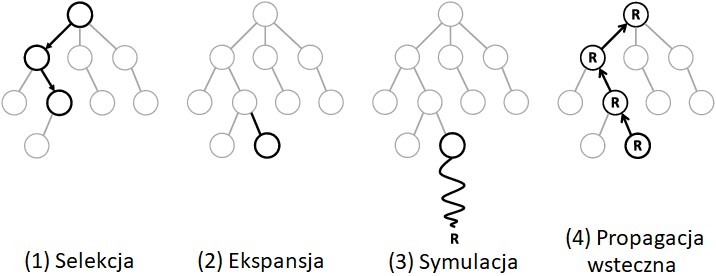
\includegraphics[width=0.8\textwidth]{mcts_phases_pl.png}
	\caption{Fazy MCTS}
	\label{rys:mcts_phases}
\end{figure}

\begin{enumerate}
	\item \textbf{Faza selekcji} (wiersz 6 w listingu) -- wybór pewnego liścia drzewa. Rozdział \ref{subsec:uct} opisuje jeden ze sposobów na wybranie wierzchołka w tej fazie.
	\item \textbf{Faza ekspansji} (wiersz 7 w listingu) -- utworzenie wierzchołków potomnych dla wierzchołka wybranego w fazie selekcji. Tworzone wierzchołki odpowiadają stanom możliwym do uzyskania przez wykonanie jednego ruchu ze stanu rodzica.
	\item \textbf{Faza symulacji} (wiersz 10 w listingu) -- rozegranie partii składającej się z losowych ruchów ze stanu jednego z wierzchołków utworzonych w poprzedniej fazie. Rozgrywana jest ona do końca, czyli do wyłonienia zwycięzcy lub spowodowania remisu, lub jest ucinana po pewnej liczbie ustalonych ruchów i wynik gry jest ewaluowany przez pewną funkcję.
	\item \textbf{Faza propagacji wstecznej} (wiersz 11 w listingu) -- aktualizacja informacji na temat wierzchołków na ścieżce od liścia, z którego rozpoczęto symulację, do korzenia drzewa. Główną przekazywaną wartością jest wynik symulacji.
\end{enumerate}

\begin{minipage}{\linewidth} % minipage to ensure listing is on seperate page
\begin{lstlisting}[caption={Pseudokod algorytmu Monte Carlo Tree Search}, label=lst:mcts, style=mystyle]
def find_next_move(curr_state):
	iterations_counter = 0
	tree = initialize_tree(curr_state)
	
	while iterations_counter < max_iterations_counter:
		curr_node = select a leaf from tree
		create child nodes from curr_node
		if curr_node has children:
			curr_node = random child of curr_node
		playout_result = simulate random playout from curr_node     
		update tree according to playout_result                     
		iterations_counter++
	
	best_state = select best child(tree.root) 
	return best_state
\end{lstlisting}
\end{minipage}


\subsection{Algorytm UCT} \label{subsec:uct}
UCT jest wariantem metody MCTS, który stara się zachować równowagę między eksploatacją bardziej obiecujących ruchów a eksploracją tych rzadko odwiedzonych. Formuła, która odpowiada za wyznaczenie najbardziej obiecującego wierzchołka w fazie wyboru MCTS jest przedstawiona jako wyrażenie (\ref{formula:uct}).

\begin{equation}\label{formula:uct}
\frac{w_i}{n_i} + c \sqrt{\frac{\ln N_i}{n_i}}
\end{equation}

W wyrażeniu (\ref{formula:uct}), indeks $i$ odnosi się do liczby wykonanych przez algorytm iteracji, czyli czterech faz MCTS. W pierwszym składniku sumy wyrażenia (\ref{formula:uct}), licznik $w_i$ oznacza sumę wszystkich wypłat w danym węźle, a mianownik $n_i$ oznacza liczbę rozegranych symulacji. Zatem ułamek ten przyjmuje wartości większe dla ruchów o większej średniej wygranej, co odpowiada ze eksploatację drzewa. Drugi składnik sumy wyrażenia (\ref{formula:uct}) przyjmuje wartości większe dla wierzchołków, dla których wykonano mniej symulacji i odpowiada eksploracji drzewa. $N_i=\sum_i n_i$, a
$c$ jest parametrem eksploracji, który może być dostosowany do badanego problemu.\\

Stworzone przez nas rozwiązanie dodaje pewne założenia do algorytmu UCT. Dodanie założeń pozwoliło nam na stworzenie rozwiązania bardziej wyspecjalizowanego -- takiego, które będzie niezależne od zasad i logiki badanych gier. 

\begin{enumerate}
	\item Rozgrywka jest prowadzona naprzemiennie przez dwóch graczy.
	\item Każdy ruch ma jednoznaczny wpływ na dalszą rozgrywkę (rozgrywka jest deterministyczna).
	\item Każdy z graczy ma dostęp do pełnej informacji o aktualnym stanie gry.
\end{enumerate}


\section{Algorytm wizualizacji drzew} \label{subsec:tree_vis}
Celem prezentowanego rozwiązania jest wizualizacja drzew w sposób najbardziej przejrzysty dla użytkownika. Ma to ułatwić poznanie struktury drzew i zależności między ich wierzchołkami. Jako że zaprojektowanie układu wierzchołków przy pewnych założeniach jest problemem NP-trudnym nawet dla drzew binarnych, co zostało wykazane w \cite{treelayout}, w prezentowanym rozwiązaniu posłużymy się heurystyką.\\

W celu uczynienia wizualizacji jak najbardziej czytelną, poczyniono pewne założenia w kontekście układu wierzchołków i krawędzi wizualizowanych drzew. Zostały one wymienione poniżej. 

\begin{enumerate}
	\item Krawędzie drzewa nie mogą się przecinać.
	\item Wierzchołki będą ustawione od góry w rzędach, a przynależność do
	rzędów będzie zależała od odległości wierzchołków od korzenia.
	\item Wierzchołki mają być narysowane możliwie najwęziej.
\end{enumerate}

W celu wyznaczenia układu wierzchołków drzewa na płaszczyźnie, który spełnia powyższe 3 założenia, skorzystano z usprawnionego algorytmu Walkera, którego złożoność czasowa jest liniowa względem liczby wierzchołków. Zaimplementowany algorytm opisany jest dokładnie w \cite{impwalkers}, a grafiki użyte w tym podrozdziale również pochodzą z tego dokumentu. Algorytm jest obszerny, jednak jego główna idea sprowadza się do podwójnego przejścia po drzewie -- tak zwanego \textit{first walk} i \textit{second walk}.

\begin{enumerate}
	\item \textit{First walk} jest przejściem po drzewie za pomocą strategii \textit{bottom-up}, a jego głównym celem jest obliczenie wstępnej współrzędnej $x$ każdego węzła. Funkcja wywołana na korzeniu drzewa wywoływana jest rekursywnie dla jego dzieci, wykonując przy tym funkcję \textit{apportion}. Następnie dzieci rozmieszczane są (współrzędna $x$) za pomocą metody \textit{execute shifts}, tak aby spełniały założenia wizualizacji, a na koniec rodzic jest umieszczany na środku w stosunku do swoich dzieci (średnia ze współrzędnych $x$ dziecka oddalonego najbardziej na lewo i na prawo). \\ Metoda \textit{apportion}, kluczowa dla algorytmu, odpowiada za łączenie nowego poddrzewa z już istniejącym poddrzewem, co jest opisane dokładniej w sekcji 3. w \cite{impwalkers}. Porównywane są wewnętrzne kontury lewego i prawego poddrzewa, czyli wierzchołki na ścieżce od korzenia do liścia, najbardziej na lewo (lub prawo) dla danego poziomu, tak jak na Rysunku \ref{rys:kontury}. Jeżeli występuje między nimi konflikt, czyli nie spełniają któregoś z wcześniej wymienionych założeń, prawe poddrzewo przesuwane jest odpowiednio za pomocą metody \textit{move subtree}. Metody \textit{execute shifts} i \textit{move subtree} aktualizują wstępnie wyliczane współrzędne $x$ wierzchołków oraz modyfikatory -- informacje o tym, o ile dany wierzchołek powinien być dodatkowo przesunięty w prawo na osi $x$, co dokładniej opisane jest w sekcji 5. w \cite{impwalkers}.
	\item \textit{Second walk} przechodzi po drzewie za pomocą strategii \textit{top-down} i rekursywnie aplikuje wyliczone końcowe współrzędne $x$ wierzchołków, sumując ich wstępnie wyliczone $x$ wraz z wyliczonymi modyfikatorami. Dodatkowo, każdy poziom rekursji oznacza poziom wierzchołka w drzewie, więc współrzędna $y$ dla każdego wierzchołka również jest zapisywana przy tym przejściu.
\end{enumerate}

Sposób rozmieszczania wierzchołków przez algorytm Walkera i końcowy efekt ilustruje Rysunek \ref{rys:spacing}.

\begin{figure}[t!]
	\centering
	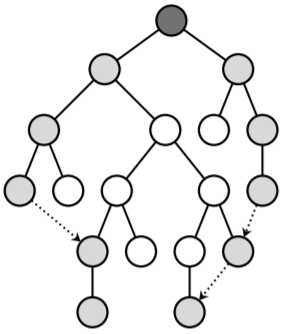
\includegraphics[width=0.3\textwidth]{kontury.png}
	\caption{Drzewo i jego kontury}
	\label{rys:kontury}
\end{figure}

\begin{figure}[t!]
	\centering
	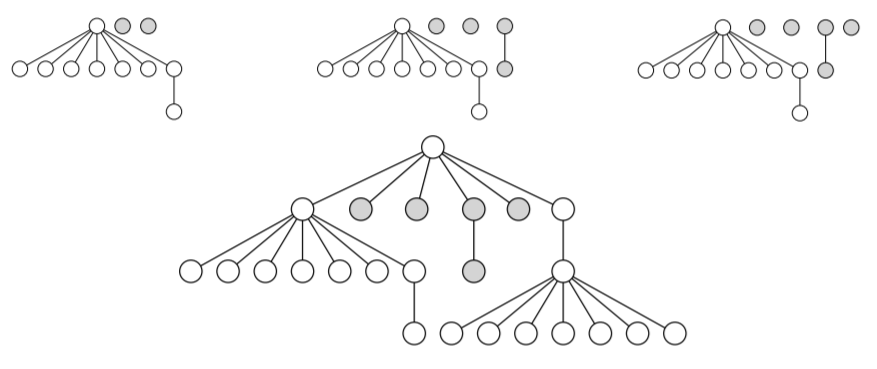
\includegraphics[width=1\textwidth]{walker-spacing.png}
	\caption{Sposób rozmieszczania wierzchołków poddrzewa}
	\label{rys:spacing}
\end{figure}